% Metódy inžinierskej práce

\documentclass[10pt,oneside,slovak,a4paper]{article}

\usepackage[slovak]{babel}
%\usepackage[T1]{fontenc}
\usepackage[IL2]{fontenc} % lepšia sadzba písmena Ľ než v T1
\usepackage[utf8]{inputenc}
\usepackage{graphicx}
\usepackage{url} % príkaz \url na formátovanie URL
\usepackage{hyperref} % odkazy v texte budú aktívne (pri niektorých triedach dokumentov spôsobuje posun textu)

\usepackage{cite}
%\usepackage{times}

\pagestyle{headings}

\title{Analýza hry Overwatch\thanks{Semestrálny projekt v predmete Metódy inžinierskej práce, ak. rok 2022/23, vedenie: Ing. Vladimír Mlynarovič, PhD.}} % meno a priezvisko vyučujúceho na cvičeniach

\author{Andrej Kotulič\\[2pt]
	{\small Slovenská technická univerzita v Bratislave}\\
	{\small Fakulta informatiky a informačných technológií}\\
	{\small \texttt{andrej.kotulic@stuba.sk}}
	}

\date{\small 6. november 2022} % upravte



\begin{document}

\maketitle

\begin{abstract}
Vzhľadom na výrazný nárast herného priemyslu v posledných rokoch a tiež na relevantnosť videohier sa tento článok zameriava na analýzu populárnej hry Overwatch (2016). 

Relevantnosť hry, okrem vplyvu na zábavný priemysel získala množstvo „game of the year“ ocenení, vďaka svojím úžasným herným mechanikám, stratégiám, rôznorodosti máp z celého sveta a veľkého množstva postáv (známych ako hrdinovia).

V tomto článku sa zameriame na základnú štruktúru hry, možnosti rôznych módov, veľkého počtu máp navrhnutých podľa reálnych destinácií na svete a postáv, ktorých je v aktuálnej hre 35. 

Taktiež sa pozrieme na esport, kde má Overwatch svoju vlastnú ligu (Overwatch League).
\end{abstract}



\section{Úvod}

Overwatch je multiplatformová „First person shooter“ hra vytvorená spoločnostou Blizzard Entertainment  v roku 2016.
Od jej vzniku si hra prešla mnoho zmenami a vylepšeniami ako zmenou herných, či odmenových mechaník.
Hra je vyvinutá pre systém PlayStation 5, PlayStation 4, Nintendo Switch, Xbox One, Xbox Series X a Series S a Microsoft Windows.

V hre sa stretnete s veľkým množstvom módov~\ref{Herné mechaniky} a obrovským množstvom máp ~\ref{Rôznorodosť máp}.

Do decembra 2022 sa v hre nachádza 36 postáv~\ref{Herné postavy} rozdelených do troch rolí:
\begin{itemize}
\item Tank
\item Damage
\item Support
\end{itemize}

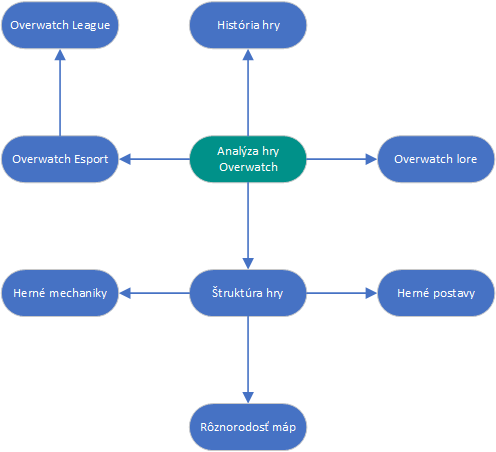
\includegraphics[scale=1]{images/struktura_temy.png}


\section{Štruktúra hry} \label{Herné mechaniky}

\subsection{Herné mechaniky} \label{Herné mechaniky}


Hra sa skladá z boja medzi dvoma tímami zložených z piatich hráčov. 

Keďže ide o hru pre viacerých hráčov, všetky postavy tímov sú skutoční hráči. Hráči v tíme spolupracujú online, aby dosiahli cieľ, ktorým môže byť zabezpečiť a brániť kontrolné body na mape alebo eskortovať náklad cez mapu v obmedzenom množstve času. Hra je značne interaktívna, pretože sa hrdinovia súčasťou rovnakého tímu automaticky zapájajú do dialógov s ostatnými hrdinami, pričom sa rozprávajú aj o mieste príbehu hry alebo o externom odkaze~\cite{Overwatchbook}.

Okrem tohto sa v hre náchádza aj niekoľko iných módov, ktoré už ale niesú tak kompetitívne. V priebehu roka sa v hre objavuje aj niekoľko speciálnych udalostí,
 kedy sú v hre dostupné nové mechaniky, módy, kozmetické predmety a úlohy.

Tieto eventy trvajú približne 3 týždne a objavujú sa poďla nasledujúceho
zoradenia: Lunar New Year, Archives, Anniversary, Summer Games, Halloween Terror a Winter Wonderland. Okrem tohto sa v hre objavuje aj niekolko mini eventov ktoré sa konajú pomedzi~\cite{Overwatchbook}.



Hra ďaľej disponuje obrovským množstvom kozmetických doplnkov ako napríklad "skiny, weapon charms, icons, sprays, voicelines, emotes". Overwatch
má aj doplnok "Highlight intro" ktorý je jedinečný pre túto hru. Ide o krátky klip najlepšieho momentu najlepšieho hráča, ktorý sa objavuje na konci kraždej hry.




\subsection{Rôznorodosť máp} \label{Rôznorodosť máp}




\subsection{Herné postavy} \label{Herné postavy}

Každá postava v hre Overwatch patrí do jednej z troch hlavných kategórií: tank, damage a support. Damage postavy sa zvyčajne zameriavajú na spôsobovanie vysokého poškodenia nepriateľskému tímu, zatiaľ čo tank postavy vynikajú ochranou svojich spojencov a držaním kľúčových miest na bojisku. Support postavy, ako už názov napovedá, poskytujú svojim spoluhráčom liečenie a ďalšie užitočné schopnosti.

Hráči môžu v priebehu zápasu prepínať medzi rôznymi postavami, čo im umožňuje prispôsobiť sa meniacim sa podmienkam v hre a čeliť stratégii nepriateľského tímu. Táto dynamická a neustále sa vyvíjajúca hrateľnosť je jedným z kľúčových prvkov, vďaka ktorým je hra Overwatch taká populárna.

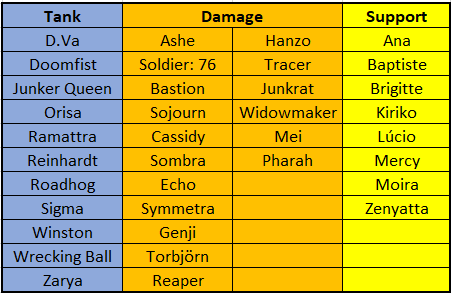
\includegraphics[scale=1.25]{images/overwatch_postavy.png}

\section{Overwatch lore} \label{Overwatch lore}

Hra sa odohráva na Zemi v blízkej budúcnosti. 

V hre sa nachádzajú roboti zvaný Omnici, ktorí boli vytvorení, aby slúžili ľudstvu ako robotníci a asistenti. Boli navrhnutí tak, aby boli všestranní, prispôsobiví a dokázali plniť širokú škálu úloh. Skupina omnikov sa však nakoniec stala sebavedomou a vytvorila kolektívne vedomie nazývané omnium. Omnium začalo masovo vyrábať omnických vojakov, čo viedlo ku globálnej kríze známej ako omnická kríza.

Po tejto kríze bola vytvorená nadnárodná jednotka Overwatch, ktorej úlohou je obnoviť mier a poriadok na svete.

Hra obsahuje rozmanité postavy, z ktorých každá má svoje jedinečné schopnosti a pôvod. Medzi hlavné postavy patrí Tracer, ktorá dokáže cestovať časom, Reinhardt, mocný rytier s masívnym raketovým kladivom, a Mercy, lekárka so schopnosťou liečiť svojich spojencov. 


\section{História hry} \label{História hry}


\section{Overwatch Esport} \label{Overwatch Esport}

Termín esports pochádza z konca deväťdesiatych rokov. V súčasnosti možno tvrdiť, že esport sa stal štandardizovaným spôsobom označovania súťažných hier v rámci a aj mimo akademickej sféri. Nie je preto prekvapujúce, že definícia esportu a jeho vzťah k športom pritiahla pozornosť výskumníkov z viacerých oblastí~\cite{Overwatchesport}.

V posledných rokoch sa herný priemysel neustále exponenciálne popularizuje, a tým aj esport priemysel sám o sebe. Zatiaľ čo pred niekoľkými rokmi by ste 
našli len málokoho, kto by čo i len vedel čo to esport je, dnes je to multimiliónová scéna s milíonmi hráčov. Pre Overwatch to platí tiež.

Overwatch mal aktívnu scénu už od jeho vzniku. Prvý veľký esport event bol World Cup 2016 na Blizzcone~\cite{Overwatchesport}.

V roku 2018 vznikla aj samostatná liga pre túto hru s názvom Overwatch league~\ref{Overwatch league - OWL}.

\subsection{Overwatch league - OWL} \label{Overwatch league - OWL}

Overwatch League je medzinárodná esportová liga pozostávajúca z 20 tímov, kde hrajú najlepší hráči Overwatch na svete. Tímy sú z miest, podobne ako vo väčšine tradičných športových líg a hoci väčšina tímov reprezentuje mestá v Spojených štátoch, existujú aj tímy, ktoré zastupujú mestá v Európe a Ázijských krajinách (dve v Európe, jedno v Južnej Kórei a štyri v Číne)~\cite{Overwatchesport}. Sezóna 2022, ktorá obsahuje novú hru Overwatch 2 PvP, začala 5. mája 2022 a končí play-off a veľkým finále neskôr v priebehu tohto roka. Vďaka špičkovej súťaži, napínavým zápletkám, rozšírenému cenovému fondu, robustným diváckym odmenám a špičkovej produkčnej hodnote je Overwatch League najlepšou esportovou ligou na svete.~\cite{Overwatchsite}.



\section{Záver} \label{zaver} % prípadne iný variant názvu



%\acknowledgement{Ak niekomu chcete poďakovať\ldots}


% týmto sa generuje zoznam literatúry z obsahu súboru literatura.bib podľa toho, na čo sa v článku odkazujete
\bibliography{literatura}
\bibliographystyle{plain} % prípadne alpha, abbrv alebo hociktorý iný
\end{document}
